% ROZDZIAŁ 17 — rozkład Lebesgue'a dowodzony niezależnie od RN
\chapter[Bezwzględna ciągłość i rozkład Lebesgue'a]{Bezwzględna ciągłość, osobliwość i rozkład Lebesgue'a miar}
\label{ch:ac-singular-17}

\providecommand{\atlasref}[2]{#2}


\section{Porównywanie miar: co znaczy, że jedna miara nie widzi więcej niż druga?}

\noindent\emph{Powiązania tematyczne w Bibliotece matematycznej:} \atlasref{P3-08::ch:girsanov}{P3-08: zastosowanie bezwzględnej ciągłości i równoważności miar w analizie stochastycznej}.

Niech $(X,\mathcal F)$ będzie przestrzenią mierzalną. Dwie miary mogą
przypisywać tym samym zbiorom różne wartości, ale istotne jest również,
czy mają te same zbiory miary zero. Zagadnienie to prowadzi do dwóch
przeciwstawnych pojęć: bezwzględnej ciągłości i wzajemnej osobliwości.
Na tym etapie nie będziemy zakładać istnienia gęstości jednej miary
względem drugiej: właśnie możliwość zbudowania takich gęstości
stanowi treść następnego rozdziału.

\begin{definicja}[Bezwzględna ciągłość miary]
\label{def:ac-measure-17}
Niech $\mu$ i $\nu$ będą miarami nieujemnymi na $(X,\mathcal F)$.
Mówimy, że $\nu$ jest \emph{bezwzględnie ciągła względem $\mu$},
i piszemy $\nu\ll\mu$, jeżeli dla każdego $E\in\mathcal F$
z warunku $\mu(E)=0$ wynika $\nu(E)=0$.
Dla skończonej miary zespolonej $\eta$ przyjmujemy tę samą definicję,
równoważnie $|\eta|\ll\mu$, gdzie $|\eta|$ jest wariacją całkowitą. Istotnie, gdy $\mu(E)=0$, wszystkie mierzalne podzbiory $E$ są zerowe względem $\mu$, więc wszystkie składniki sum wyznaczających $|\eta|(E)$ są zerowe. Kierunek odwrotny wynika z $|\eta(E)|\le|\eta|(E)$.
\end{definicja}

\begin{uwaga}[Dlaczego warunki dla miary zespolonej są równoważne?]
Jeżeli $\mu(E)=0$, to $\mu(A)=0$ dla każdego mierzalnego $A\subseteq E$.
Stąd $\eta(A)=0$, a z definicji wariacji jako supremum sum po podziałach
wynika $|\eta|(E)=0$. Odwrotna implikacja wynika z
$|\eta(E)|\le|\eta|(E)$. Sam warunek $\eta(E)=0$ dla jednego,
ustalonego $E$ nie oznacza jednak $|\eta|(E)=0$.
\end{uwaga}

\begin{przyklad}[Miara określona gęstością]
\label{ex:ac-density-17}
Dla dowolnej miary $\mu$ i mierzalnej funkcji $f:X\to[0,\infty]$
miara $\nu_f(E)=\int_E f(x)\,\mathrm d\mu(x)$ jest bezwzględnie
ciągła względem $\mu$, nawet jeśli $\nu_f(X)=\infty$.
W przypadku zespolonego $f\in L^1(\mu)$ analogiczna własność
wynika z twierdzenia~\ref{thm:density-variation-16}.
Nie wyciągamy jeszcze wniosku odwrotnego: $\nu\ll\mu$
samo w sobie nie jest \emph{definicją} istnienia gęstości.
\end{przyklad}

\begin{przyklad}[Miary Diraca a miara Lebesgue'a]
Na $(\mathbb R,\mathcal L_1)$ oznaczmy przez $\delta_a$ miarę Diraca
w punkcie $a\in\mathbb R$. Wówczas $\delta_a\not\ll\lambda_1$,
ponieważ $\lambda_1(\{a\})=0$, lecz $\delta_a(\{a\})=1$.
Z drugiej strony $\lambda_1\not\ll\delta_a$, gdyż
$\delta_a(\mathbb R\setminus\{a\})=0$ i
$\lambda_1(\mathbb R\setminus\{a\})=\infty$.
\end{przyklad}

\begin{definicja}[Wzajemna równoważność miar]
\label{def:equivalent-measures-17}
Dwie nieujemne miary $\mu,\nu$ na $(X,\mathcal F)$ nazywamy
\emph{równoważnymi}, co zapisujemy $\mu\sim\nu$,
jeśli $\mu\ll\nu$ oraz $\nu\ll\mu$.
Znaczy to dokładnie, że mają te same mierzalne zbiory miary zero.
\end{definicja}

\begin{przyklad}[Równoważne miary nie muszą być równe]
Na $X=(0,1)$ miary $\mu=\lambda_1|_X$ i
$\nu(E)=\int_E x\,\mathrm d\lambda_1(x)$ są równoważne,
ponieważ $x>0$ na $X$. Istotnie, $\mu(E)=0$
implikuje $\nu(E)=0$. Odwrotnie, jeśli $\nu(E)=0$,
to dla $E_n=E\cap\{x\ge1/n\}$ mamy
$\mu(E_n)\le n\int_{E_n}x\,\mathrm d\lambda_1(x)=0$.
Ponieważ $E=\bigcup_{n\ge1}E_n$, również $\mu(E)=0$.
Miary te nie są równe: $\mu(X)=1$, zaś $\nu(X)=1/2$.
Zmiana wagi może zachować wszystkie zbiory zerowe,
lecz zmienić wartości miar.
\end{przyklad}

\section{Wzajemna osobliwość i przykłady}
Pojęcie wzajemnej osobliwości wprowadziliśmy już w
definicji~\ref{def:singular-16}. Powtórzymy je w postaci dogodnej
do badania rozkładów.

Przypominamy definicję~\ref{def:singular-16}:
dwie nieujemne miary $\nu,\mu$ na $(X,\mathcal F)$ są
\emph{wzajemnie osobliwe}, $\nu\perp\mu$, gdy istnieje
$S\in\mathcal F$ takie, że $\mu(S)=0$ i
$\nu(X\setminus S)=0$. Dla miary zespolonej $\eta$
piszemy $\eta\perp\mu$, gdy $|\eta|\perp\mu$.
Jest to rozszerzenie tej samej relacji na miary zespolone,
a nie nowa definicja dla miar nieujemnych.

Zbiór $S$ w definicji jest \emph{zbiorem skupiającym}
miarę $\nu$ (można też mówić o mierzalnym nośniku). Nie należy mylić go z
\emph{nośnikiem topologicznym}: ten drugi wymaga topologii
i jest definiowany za pomocą otoczeń punktów.

\begin{lemat}[Elementarne własności osobliwości]
\label{lem:singularity-17}
Niech $\mu,\nu,\rho$ będą miarami nieujemnymi na $(X,\mathcal F)$.
Wtedy:
\begin{enumerate}[label=\textup{(\roman*)}]
\item $\nu\perp\mu$ wtedy i tylko wtedy, gdy $\mu\perp\nu$;
\item jeśli $\nu\ll\mu$ i $\nu\perp\mu$, to $\nu=0$;
\item jeśli $\nu\perp\mu$ oraz $\rho\perp\mu$, to
$\nu+\rho\perp\mu$;
\item dla dowolnego $S\in\mathcal F$ miary
$\mu|_S(E):=\mu(E\cap S)$ i
$\mu|_{X\setminus S}(E):=\mu(E\setminus S)$ są wzajemnie osobliwe.
\end{enumerate}
\end{lemat}
\begin{proof}
(i) Jeśli $\mu(S)=0$ i $\nu(X\setminus S)=0$, to
$X\setminus S$ świadczy o relacji odwrotnej.
(ii) Z $\nu\ll\mu$ wynika $\nu(S)=0$, a z osobliwości
$\nu(X\setminus S)=0$, więc $\nu(X)=0$ i $\nu=0$.
(iii) Jeśli $\nu$ jest skupiona na $S$, a $\rho$ na $T$,
to $\mu(S\cup T)=0$ i $(\nu+\rho)(X\setminus(S\cup T))=0$.
(iv) Pierwsza miara jest skupiona na $S$, a druga na $X\setminus S$.
\end{proof}

\begin{przyklad}[Miara dyskretna i miara ciągła]
Niech $(a_n)_{n\ge1}$ będzie ciągiem punktów w $\mathbb R$, a
$(c_n)_{n\ge1}$ ciągiem liczb nieujemnych o
$\sum_nc_n<\infty$. Miara $\nu=\sum_nc_n\delta_{a_n}$
jest osobliwa względem $\lambda_1$: wystarczy
$S=\{a_n:n\ge1\}$, zbiór przeliczalny, więc zerowy
względem miary Lebesgue'a. Nie ma znaczenia, czy $S$ jest
gęsty w $\mathbb R$.
\end{przyklad}

\section{Kryterium epsilon--delta i rola skończoności}
Warunek $\nu\ll\mu$ mówi jedynie o zbiorach dokładnie zerowej
miary. Gdy $\nu$ jest skończona, można go wzmocnić do
\emph{jednostajnej} kontroli małych zbiorów.

\begin{twierdzenie}[Kryterium epsilon--delta]
\label{thm:eps-delta-ac-17}
Niech $\mu$ będzie dowolną miarą nieujemną na $(X,\mathcal F)$,
a $\nu$ miarą nieujemną o $\nu(X)<\infty$.
Następujące warunki są równoważne:
\begin{enumerate}[label=\textup{(\roman*)}]
\item $\nu\ll\mu$;
\item dla każdego $\varepsilon>0$ istnieje $\delta>0$ taka,
że dla każdego $E\in\mathcal F$ zachodzi implikacja
$\mu(E)<\delta\implies\nu(E)<\varepsilon$.
\end{enumerate}
Dla skończonej miary zespolonej $\eta$ równoważność zachodzi po
zastąpieniu $\nu(E)$ przez $|\eta|(E)$.
\end{twierdzenie}
\begin{proof}
(ii)$\Rightarrow$(i). Jeśli $\mu(E)=0$, to
$\mu(E)<\delta$ dla każdej liczby $\delta>0$.
Stąd $\nu(E)<\varepsilon$ dla każdego $\varepsilon>0$,
a więc $\nu(E)=0$.

(i)$\Rightarrow$(ii). Gdyby (ii) było fałszywe, istniałoby
$\varepsilon_0>0$ takie, że dla każdego $n\ge1$
można wybrać $E_n\in\mathcal F$ z
$\mu(E_n)<2^{-n}$ oraz $\nu(E_n)\ge\varepsilon_0$.
Niech $F_m=\bigcup_{n\ge m}E_n$ i
$F=\bigcap_{m\ge1}F_m=\limsup_nE_n$.
Z przeliczalnej podaddytywności otrzymujemy
$\mu(F_m)\le\sum_{n\ge m}2^{-n}$,
zatem $\mu(F)=0$. Każdy $F_m$ zawiera $E_m$, więc
$\nu(F_m)\ge\varepsilon_0$. Ponieważ $F_m\downarrow F$
i $\nu(F_1)\le\nu(X)<\infty$, ciągłość miary z góry daje
$\nu(F)=\lim_m\nu(F_m)\ge\varepsilon_0$.
Przeczy to $\nu\ll\mu$. W przypadku zespolonym
stosujemy wynik do skończonej miary $|\eta|$.
\end{proof}

\begin{uwaga}[Dlaczego skończoności $\nu$ nie wolno pominąć?]
Na $X=(0,1)$ z miarą $\mu=\lambda_1$ określmy
$\nu(E)=0$ dla $\mu(E)=0$ oraz $\nu(E)=\infty$
dla $\mu(E)>0$. Jest to miara: dla rozłącznych
$(E_n)$ suma $\sum_n\nu(E_n)$ jest równa $0$ wtedy
i tylko wtedy, gdy wszystkie $E_n$ są zerowe; w przeciwnym
razie jest równa $\infty$. Mamy $\nu\ll\mu$,
ale nie zachodzi warunek epsilon--delta, bo przedziały
o dowolnie małej dodatniej długości mają $\nu(E)=\infty$.
\end{uwaga}

\begin{wniosek}[Ciągłość całki względem zbioru całkowania]
\label{cor:uniform-abs-cont-int-17}
Niech $f\in L^1(\mu)$ na dowolnej przestrzeni z miarą.
Wtedy dla każdego $\varepsilon>0$ istnieje $\delta>0$ taka,
że $\mu(E)<\delta$ implikuje
$\int_E|f(x)|\,\mathrm d\mu(x)<\varepsilon$.
\end{wniosek}
\begin{proof}
Miara $E\mapsto\int_E|f|\,\mathrm d\mu(x)$ jest skończona
i bezwzględnie ciągła względem $\mu$, zatem stosujemy
poprzednie twierdzenie.
\end{proof}

\section{Rozkład Lebesgue'a: przypadek miar skończonych}
\begin{twierdzenie}[Rozkład Lebesgue'a dla miar skończonych]
\label{thm:lebesgue-decomp-finite-17}
Niech $\mu$ i $\nu$ będą skończonymi miarami nieujemnymi
na tej samej przestrzeni mierzalnej $(X,\mathcal F)$.
Istnieje dokładnie jedna para miar nieujemnych
$(\nu_{\mathrm{ac}},\nu_{\mathrm{s}})$ taka, że
\begin{equation}\label{eq:decomp-finite-17}
\nu=\nu_{\mathrm{ac}}+\nu_{\mathrm{s}},\qquad
\nu_{\mathrm{ac}}\ll\mu,\qquad \nu_{\mathrm{s}}\perp\mu.
\end{equation}
Obie składowe są skończone. W dowodzie nie korzystamy
z twierdzenia Radona--Nikodyma.
\end{twierdzenie}
\begin{proof}
\emph{Konstrukcja.} Dla każdego $k\ge1$ stosujemy rozkład
Hahna (twierdzenie~\ref{thm:hahn-16}) do skończonej miary
ze znakiem $\nu-2^k\mu$. Otrzymujemy rozłączne zbiory
$P_k,N_k\in\mathcal F$ takie, że
$P_k\cup N_k=X$ oraz
\begin{equation}\label{eq:ineq-hahn-decomp-17}
\nu(A)\ge2^k\mu(A)\quad(A\subseteq P_k),\qquad
\nu(B)\le2^k\mu(B)\quad(B\subseteq N_k)
\end{equation}
dla wszystkich mierzalnych $A,B$. W szczególności
$\mu(P_k)\le2^{-k}\nu(P_k)\le2^{-k}\nu(X)$.
Definiujemy
\[
S=\limsup_{k\to\infty}P_k
  =\bigcap_{m\ge1}\bigcup_{k\ge m}P_k.
\]
Ponieważ $\sum_k\mu(P_k)<\infty$, lemat
Borela--Cantellego (lub bezpośrednia podaddytywność)
daje $\mu(S)=0$.

Dla każdego $x\in X\setminus S$ istnieje $m$ takie,
że $x\notin P_k$ dla wszystkich $k\ge m$.
W szczególności
$X\setminus S\subseteq\bigcup_{k\ge1}N_k$.
Jeśli $E\in\mathcal F$ i $\mu(E)=0$, to z drugiej
nierówności w \eqref{eq:ineq-hahn-decomp-17} wynika
$\nu(E\cap N_k)=0$ dla każdego $k$.
Zatem $\nu(E\setminus S)=0$.
Kładziemy
$\nu_{\mathrm{s}}(A)=\nu(A\cap S)$ oraz
$\nu_{\mathrm{ac}}(A)=\nu(A\setminus S)$
dla wszystkich $A\in\mathcal F$.
Obie funkcje są skończonymi miarami nieujemnymi,
a ich suma jest równa $\nu$.
Miara $\nu_{\mathrm{s}}$ jest skupiona na $S$,
przy $\mu(S)=0$, a z poprzedniego akapitu
wynika $\nu_{\mathrm{ac}}\ll\mu$.

\emph{Jednoznaczność.} Załóżmy, że
$\nu=\alpha+\sigma=\alpha'+\sigma'$,
gdzie $\alpha,\alpha'\ll\mu$ oraz
$\sigma,\sigma'\perp\mu$. Niech $T,T'$ będą
mierzalnymi zbiorami $\mu$-zerowymi skupiającymi
odpowiednio $\sigma,\sigma'$, i niech $Z=T\cup T'$.
Wówczas $\mu(Z)=0$, zatem $\alpha(Z)=\alpha'(Z)=0$.
Na $X\setminus Z$ mamy $\sigma=\sigma'=0$,
a więc dla każdego $A\in\mathcal F$
$\alpha(A\setminus Z)=\nu(A\setminus Z)=\alpha'(A\setminus Z)$.
Ponieważ obie miary $\alpha,\alpha'$ zerują się na $Z$,
wynika $\alpha=\alpha'$ i następnie $\sigma=\sigma'$.
\end{proof}

\begin{uwaga}[Dlaczego ten dowód nie jest kołowy?]
Użyliśmy wyłącznie rozkładu Hahna dla skończonych miar ze
znakiem, oszacowania szeregu $\sum_k2^{-k}$ oraz ciągłości
miary. Nie korzystaliśmy z reprezentacji przez gęstość.
Dopiero twierdzenie Radona--Nikodyma pokaże, że składową
$\nu_{\mathrm{ac}}$ można zapisać jako całkę funkcji.
\end{uwaga}

\section{Rozkład Lebesgue'a dla miar sigma-skończonych}
\begin{twierdzenie}[Rozkład Lebesgue'a w przypadku $\sigma$-skończonym]
\label{thm:lebesgue-decomp-sigfin-17}
Niech $\mu$ i $\nu$ będą miarami nieujemnymi,
$\sigma$-skończonymi na $(X,\mathcal F)$.
Wtedy istnieje dokładnie jedna para miar nieujemnych
$\nu_{\mathrm{ac}},\nu_{\mathrm{s}}$, spełniająca
$\nu=\nu_{\mathrm{ac}}+\nu_{\mathrm{s}}$,
$\nu_{\mathrm{ac}}\ll\mu$ i $\nu_{\mathrm{s}}\perp\mu$.
Obie składowe są $\sigma$-skończone.
\end{twierdzenie}
\begin{proof}
Wybieramy mierzalne pokrycia
$X=\bigcup_iA_i=\bigcup_jB_j$ takie, że
$\mu(A_i)<\infty$ i $\nu(B_j)<\infty$.
Rodzina $(A_i\cap B_j)_{i,j\ge1}$ jest przeliczalnym
pokryciem $X$ przez zbiory mające skończoną miarę
względem obu miar. Po uporządkowaniu tej rodziny
i odejmowaniu wcześniejszych zbiorów uzyskujemy
mierzalny, parami rozłączny podział $X=\bigsqcup_{n\ge1}C_n$
z $\mu(C_n),\nu(C_n)<\infty$.

Na każdym $C_n$, wyposażonym w $\sigma$-algebrę śladową,
stosujemy twierdzenie~\ref{thm:lebesgue-decomp-finite-17}.
Niech $S_n\subseteq C_n$ będzie zbiorem o
$\mu(S_n)=0$, na którym skupia się część osobliwa
ograniczenia $\nu|_{C_n}$, a na $C_n\setminus S_n$
miara $\nu|_{C_n}$ jest bezwzględnie ciągła względem
$\mu|_{C_n}$. Przyjmujemy $S=\bigcup_nS_n$.
Ponieważ $\mu(S)=0$, miara
$\nu_{\mathrm{s}}(E):=\nu(E\cap S)$ jest osobliwa.
Jeśli $\mu(E)=0$, to
$\nu((E\setminus S)\cap C_n)=0$ dla każdego $n$;
przeliczalna addytywność daje $\nu(E\setminus S)=0$.
Zatem $\nu_{\mathrm{ac}}(E):=\nu(E\setminus S)$
jest bezwzględnie ciągła względem $\mu$.
Składowe są $\sigma$-skończone, gdyż dominują je
ograniczenia $\nu$ na zbiorach $B_j$.
Jednoznaczność dowodzi się dokładnie tak jak
w przypadku skończonym, bez użycia skończoności masy.
\end{proof}

\begin{wniosek}[Rozkład miary zespolonej]
\label{cor:complex-lebesgue-decomp-17}
Niech $\mu$ będzie nieujemną miarą $\sigma$-skończoną,
a $\eta$ skończoną miarą zespoloną na $(X,\mathcal F)$.
Wtedy istnieje dokładnie jedna para miar zespolonych
$\eta_{\mathrm{ac}}$ i $\eta_{\mathrm{s}}$ taka, że
$\eta=\eta_{\mathrm{ac}}+\eta_{\mathrm{s}}$,
$\eta_{\mathrm{ac}}\ll\mu$ oraz $\eta_{\mathrm{s}}\perp\mu$.
\end{wniosek}
\begin{proof}
Stosujemy twierdzenie~\ref{thm:lebesgue-decomp-sigfin-17}
do nieujemnej skończonej miary $|\eta|$, otrzymując
zbiór $S$ o $\mu(S)=0$, taki że
$|\eta||_{X\setminus S}\ll\mu$.
Definiujemy $\eta_{\mathrm{s}}(E)=\eta(E\cap S)$
oraz $\eta_{\mathrm{ac}}(E)=\eta(E\setminus S)$.
Dla każdego $E$ wariacja ograniczenia $\eta|_S$
nie przekracza $|\eta|(E\cap S)$, co dowodzi osobliwości;
podobnie $|\eta_{\mathrm{ac}}|(E)\le|\eta|(E\setminus S)$,
co daje bezwzględną ciągłość.
Dla jednoznaczności bierzemy sumę zbiorów
$\mu$-zerowych skupiających dwie hipotetyczne części
osobliwe i powtarzamy argument z dowodu twierdzenia
\ref{thm:lebesgue-decomp-finite-17}, z uwzględnieniem
zerowości części bezwzględnie ciągłych na tych zbiorach.
\end{proof}

\section{Co może być składową osobliwą?}
\begin{przyklad}[Rozkład dyskretno-ciągły]
Na $X=(0,1)$ z miarą $\mu=\lambda_1|_X$ określmy
\[
\nu(E)=\int_E(1+x)\,\mathrm d\lambda_1(x)
       +3\delta_{1/3}(E)+2\delta_{2/3}(E).
\]
Wtedy $\nu_{\mathrm{ac}}(E)=\int_E(1+x)\,\mathrm d\lambda_1(x)$,
a $\nu_{\mathrm{s}}=3\delta_{1/3}+2\delta_{2/3}$.
Jest to rozkład Lebesgue'a: część osobliwa jest skupiona
na dwuelementowym zbiorze miary Lebesgue'a zero.
\end{przyklad}

\begin{przyklad}[Miara Cantora — osobliwość bez atomów]
\label{ex:cantor-measure-17}
Podamy konstrukcję niewymagającą wcześniejszego twierdzenia
o miarach Lebesgue'a--Stieltjesa. Dla $x\in[0,1)$ niech
\[
b_n(x)=\lfloor2^nx\rfloor-2\lfloor2^{n-1}x\rfloor\in\{0,1\},
\qquad n\ge1.
\]
Są to cyfry rozwinięcia dwójkowego, przy czym dla liczb
dwójkowo wymiernych przyjęliśmy rozwinięcie zakończone
samymi zerami. Określamy
$T(x)=\sum_{n\ge1}2b_n(x)3^{-n}$ dla $x\in[0,1)$
oraz $T(1)=1$. Każda funkcja $b_n$ jest borelowska,
a szereg definiujący $T$ jest jednostajnie zbieżny,
więc $T:[0,1]\to[0,1]$ jest borelowska. Jej wartości
należą do środkowego zbioru Cantora $C$, ponieważ ich
rozwinięcia trójkowe używają wyłącznie cyfr $0$ i $2$.

Niech $\kappa=T_*(\lambda_1|_{[0,1]})$. Jest to miara
probabilistyczna, $\kappa(C)=1$. Na poziomie $n$ konstrukcji zbioru Cantora
każdy z $2^n$ rozłącznych przedziałów podstawowych
$I_{\varepsilon_1,\ldots,\varepsilon_n}$ odpowiada
słowu $(\varepsilon_1,\ldots,\varepsilon_n)\in\{0,1\}^n$:
jego lewy koniec to $\ell=\sum_{j=1}^n2\varepsilon_j3^{-j}$,
a prawy to $\ell+3^{-n}$. Jeśli pierwsze $n$ cyfr
$b_j(x)$ tworzą to słowo, pozostały ogon szeregu dla
$T(x)$ należy do $[0,3^{-n}]$, więc $T(x)\in
I_{\varepsilon_1,\ldots,\varepsilon_n}$. Odwrotnie,
gdy słowo jest inne, $T(x)$ należy do innego przedziału
poziomu $n$, rozłącznego z rozpatrywanym.
Dla $x<1$ teleskopowanie definicji cyfr daje
$\lfloor2^nx\rfloor=\sum_{j=1}^n b_j(x)2^{n-j}$,
gdyż $\lfloor x\rfloor=0$.
Zatem przeciwobraz danego przedziału podstawowego
w $[0,1)$ jest dokładnie przedziałem dwójkowym
$[k2^{-n},(k+1)2^{-n})$, gdzie
$k=\sum_{j=1}^n\varepsilon_j2^{n-j}$.
Punkt $1$ nie wpływa na miarę przeciwobrazu. Stąd
$\kappa(I_{\varepsilon_1,\ldots,\varepsilon_n})=2^{-n}$.
Każdy $y\in C$ należy na każdym poziomie do jednego
takiego przedziału, zatem
$\kappa(\{y\})\le2^{-n}$ dla wszystkich $n$ i
$\kappa(\{y\})=0$. Dla $y\notin C$ mamy
$\kappa(\{y\})=0$, gdyż $\kappa$ jest skupiona na $C$.
Z twierdzenia \ref{thm:atomic-cont-singular-17} wynika więc, że $\kappa$ jest bezatomowa. Ponieważ
$\lambda_1(C)=0$ (zbiór $C$ zawiera się na każdym poziomie $n$ w $2^n$ przedziałach długości $3^{-n}$, o łącznej długości $(2/3)^n$), otrzymujemy $\kappa\perp\lambda_1$.
Pokazuje to, że \emph{osobliwość} nie jest tym samym co
\emph{dyskretność}. Dystrybuanta $x\mapsto\kappa((-\infty,x])$ jest ciągła dzięki brakowi atomów, niemalejąca, ma wartości $0$ i $1$ na końcach $[0,1]$, a na każdej luce zbioru Cantora jest stała. Jeśli $I=[\ell,r]$ jest $k$-tym przedziałem
podstawowym poziomu $n$, licząc od lewej od $k=0$,
to dystrybuanta przyjmuje wartości $k2^{-n}$ w $\ell$
i $(k+1)2^{-n}$ w $r$: przedziały wcześniejsze mają
łącznie masę $k2^{-n}$, a singletony mają masę zero.
Są to wartości klasycznej funkcji Cantora. Końce
przedziałów podstawowych są gęste w zbiorze Cantora,
gdyż każdy jego punkt znajduje się w przedziale
długości $3^{-n}$ na każdym poziomie. Zatem wartości
na końcach wyznaczają dystrybuantę jednoznacznie
przez ciągłość na zbiorze Cantora i stałość w lukach.
Pochodna dystrybuanty jest zerowa w każdej otwartej
luce, a suma luk ma pełną miarę Lebesgue'a w $[0,1]$.
Dystrybuanta nie jest jednak bezwzględnie ciągła:
gdyby była, wzór Newtona--Leibniza dla funkcji
bezwzględnie ciągłych
(twierdzenie \atlasref{AM1-37::it:thm:ac-lebesgue-primitive}{AM I-36: wzór Newtona--Leibniza})
dawałby różnicę wartości końcowych równą zero zamiast $1$.
\end{przyklad}

W dalszych przykładach oznaczamy funkcję Cantora przez $C$, środkowotrzeci zbiór Cantora przez $K$, a skonstruowaną miarę przez $\mu_C=\kappa$.

\begin{figure}[htbp]
\centering
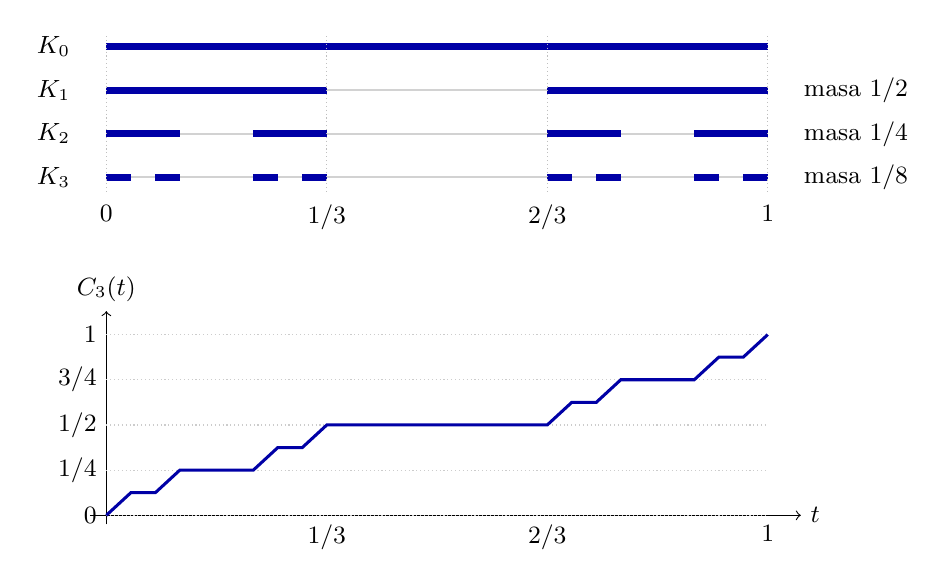
\begin{tikzpicture}[x=8.4cm,y=0.85cm,font=\small]
 \foreach \n/\yy in {0/0,1/-0.65,2/-1.3,3/-1.95}{
   \node[anchor=east] at (-0.04,\yy) {$K_{\n}$};
   \draw[gray!35,line width=0.7pt] (0,\yy)--(1,\yy);
 }
 \foreach \left/\right/\yy in {0/1/0,0/{1/3}/-0.65,{2/3}/1/-0.65,
  0/{1/9}/-1.3,{2/9}/{1/3}/-1.3,{2/3}/{7/9}/-1.3,{8/9}/1/-1.3,
  0/{1/27}/-1.95,{2/27}/{3/27}/-1.95,{6/27}/{7/27}/-1.95,{8/27}/{9/27}/-1.95,
  {18/27}/{19/27}/-1.95,{20/27}/{21/27}/-1.95,{24/27}/{25/27}/-1.95,{26/27}/1/-1.95}{
    \draw[blue!65!black,line width=2.6pt] ({\left},\yy)--({\right},\yy);
 }
 \foreach \xx/\txt in {0/0,{1/3}/{1/3},{2/3}/{2/3},1/1}{
  \draw[gray!50,densely dotted] ({\xx},0.16)--({\xx},-2.18);
  \node[below] at ({\xx},-2.22) {$\txt$};
 }
 \node[anchor=west,align=left] at (1.04,-0.65) {masa $1/2$};
 \node[anchor=west,align=left] at (1.04,-1.3) {masa $1/4$};
 \node[anchor=west,align=left] at (1.04,-1.95) {masa $1/8$};
 \begin{scope}[shift={(0,-7.0)},yscale=2.7]
 \draw[->] (-0.025,0)--(1.05,0) node[right] {$t$};
 \draw[->] (0,-0.05)--(0,1.13) node[above] {$C_3(t)$};
 \foreach \yy/\txt in {0/0,{1/4}/{1/4},{1/2}/{1/2},{3/4}/{3/4},1/1}{
  \draw[gray!40,densely dotted] (0,{\yy})--(1,{\yy});
  \node[left] at (0,{\yy}) {$\txt$};
 }
 \foreach \xx/\txt in {{1/3}/{1/3},{2/3}/{2/3},1/1}{
  \node[below] at ({\xx},0) {$\txt$};
 }
 \draw[blue!65!black,line width=1.1pt]
 (0,0)--({1/27},{1/8})--({2/27},{1/8})--({3/27},{1/4})
 --({6/27},{1/4})--({7/27},{3/8})--({8/27},{3/8})--({9/27},{1/2})
 --({18/27},{1/2})--({19/27},{5/8})--({20/27},{5/8})--({21/27},{3/4})
 --({24/27},{3/4})--({25/27},{7/8})--({26/27},{7/8})--(1,1);
 \end{scope}
\end{tikzpicture}
\caption{Pierwsze etapy konstrukcji zbioru Cantora $K_n$ (u góry);
podana masa dotyczy pojedynczego niebieskiego przedziału.
U dołu: $C_3$, ciągłe odcinkami afiniczne przybliżenie funkcji Cantora $C$,
zgodne z nią na końcach przedziałów poziomu trzeciego i stałe na
usuniętych lukach. Nie jest to wykres samej funkcji granicznej.}
\label{it:fig:cantor-construction}
\end{figure}

Niech $K_n$ oznacza sumę przedziałów podstawowych
poziomu $n$ (w szczególności $K_0=[0,1]$).
Na rysunku \ref{it:fig:cantor-construction} przedstawiono
pierwsze trzy etapy. Funkcja $C_n$ zgodna z $C$ na
końcach przedziałów poziomu $n$, afiniczna na tych
przedziałach i stała na lukach, przybliża $C$
jednostajnie: na każdym przedziale podstawowym
obie funkcje przyjmują wartości pomiędzy tymi samymi
wartościami końcowymi, których różnica wynosi $2^{-n}$,
a w lukach są równe. Stąd $\|C_n-C\|_\infty\le 2^{-n}$.

\begin{twierdzenie}[Samopodobieństwo i całkowanie względem miary Cantora]
\label{it:thm:cantor-selfsimilar-integrals}
Niech $S_0(t)=t/3$ oraz $S_1(t)=(t+2)/3$ dla $t\in[0,1]$.
Wówczas
\[
 \mu_C=\tfrac12(S_0)_*\mu_C+\tfrac12(S_1)_*\mu_C.
\]
Dla każdej nieujemnej funkcji borelowskiej $f:[0,1]\to[0,+\infty]$
oraz dla każdej funkcji borelowskiej całkowalnej względem
$\mu_C$ zachodzi
\[
 \int f\,\mathrm d\mu_C=
 \tfrac12\int f(t/3)\,\mathrm d\mu_C(t)
 +\tfrac12\int f((t+2)/3)\,\mathrm d\mu_C(t).
\]
W przypadku funkcji całkowalnej oba składniki po prawej
stronie są skończonymi całkami.
\end{twierdzenie}
\begin{proof}
Dla $x\in[0,1)$ kładziemy $j=\lfloor2x\rfloor$ oraz
$u=2x-j\in[0,1)$. Z definicji cyfr dwójkowych
$b_1(x)=j$ i $b_{n+1}(x)=b_n(u)$ dla $n\ge1$:
w różnicy
$\lfloor2^{n+1}x\rfloor-2\lfloor2^nx\rfloor$
składniki zawierające $j$ znoszą się po podstawieniu
$x=(u+j)/2$. Stąd
$T(x)=(2j+T(u))/3=S_j(T(u))$.
Dla borelowskiego $A\subset[0,1]$ przeciwobraz
$T^{-1}(A)$ na połowie $[j/2,(j+1)/2)$ jest obrazem
zbioru $\{u\in[0,1): S_j(T(u))\in A\}$ przez
odwzorowanie $u\mapsto(u+j)/2$. Miara Lebesgue'a
tego obrazu jest połową miary zbioru wyjściowego.
Punkt $1$ ma miarę zero, więc sumując po $j=0,1$,
otrzymujemy
\[
 \mu_C(A)=\tfrac12\mu_C(S_0^{-1}(A))
          +\tfrac12\mu_C(S_1^{-1}(A)).
\]
To jest żądana równość miar.
Wzór całkowy dla funkcji charakterystycznych jest
dokładnie tą równością. Dla funkcji prostych nieujemnych
wynika z liniowości, a dla dowolnych funkcji nieujemnych
z aproksymacji rosnącym ciągiem funkcji prostych i
twierdzenia \atlasref{ME-08::thm:mct}{ME-08: twierdzenie Beppo Leviego} o zbieżności monotonicznej.
Dla funkcji całkowalnych stosujemy najpierw wzór
do $|f|$, aby uzyskać całkowalność obu złożeń.
Rozkład na części dodatnią i ujemną, a dla funkcji
zespolonych również na rzeczywistą i urojoną,
daje wzór w pozostałych przypadkach.
\end{proof}

\begin{przyklad}[Momenty miary osobliwej]
\label{it:ex:cantor-moments}
Oznaczmy $m_n=\int_{[0,1]}t^n\,\mathrm d\mu_C(t)$
dla $n\ge0$. Wszystkie momenty są skończone, gdyż
$0\le t^n\le1$ i $\mu_C$ jest probabilistyczna.
Mamy $m_0=1$. Z twierdzenia
\ref{it:thm:cantor-selfsimilar-integrals} i wzoru dwumianowego
dla $n\ge1$ otrzymujemy
\[
 m_n=\frac{1}{2\cdot3^n}
       \left(m_n+\sum_{k=0}^n\binom{n}{k}2^{n-k}m_k\right),
 \qquad
 m_n=\frac{\sum_{k=0}^{n-1}\binom{n}{k}2^{n-k}m_k}
               {2(3^n-1)}.
\]
W drugim wzorze przenieśliśmy oba wyrazy zawierające
$m_n$ na lewą stronę i podzieliliśmy przez dodatni
współczynnik. Rekurencja daje $m_1=2/4=1/2$,
$m_2=(4+4m_1)/16=3/8$ oraz
$m_3=(8+12m_1+6m_2)/52=5/16$.
Z kryterium całkowalności Riemanna--Stieltjesa (\atlasref{MA1-40::it:thm:rs-oscillation}{MA1-40}) oraz zgodności z całką względem miary (\atlasref{MA1-42::tw:ks-measure}{MA1-42}) dla funkcji
ciągłych całki Riemanna--Stieltjesa względem $C$
są równe całkom względem $\mu_C$ (brak masy w $0$
pozwala całkować po $[0,1]$ zamiast $(0,1]$).
W szczególności
\[
\int_0^1 1\,\mathrm dC=1,\qquad \int_0^1 x\,\mathrm dC=\frac12,\qquad \int_0^1 x^2\,\mathrm dC=\frac38.
\]
Ponadto z całkowania przez części (twierdzenie \atlasref{MA1-40::it:thm:rs-tools}{MA1-40}), ponieważ $C$ jest ciągła i ma wahanie ograniczone, wynika $2\int_0^1 C\,\mathrm dC=C(1)^2-C(0)^2=1$. Choć $C'=0$ prawie wszędzie, nie wolno zastępować $\mathrm dC$ przez $C'(x)\,\mathrm dx$: zgubilibyśmy część osobliwą miary. Wszystkie funkcje podcałkowe w tym przykładzie są
ciągłe, więc podane równości obowiązują dla całek
Riemanna--Stieltjesa, Lebesgue'a--Stieltjesa i
Kurzweila--Stieltjesa (twierdzenie \atlasref{MA1-42::tw:ks-measure}{MA1-42}).
\end{przyklad}


\begin{uwaga}[Trzy składniki klasycznego rozkładu na prostej]
Dla skończonej miary borelowskiej na $\mathbb R$ część
osobliwą można dalej rozdzielić na część atomową,
skupioną na przeliczalnym zbiorze, oraz część osobliwą
bezatomową. Zatem otrzymujemy składowe: bezwzględnie
ciągłą, osobliwą atomową i osobliwą bezatomową.
To \emph{dalszy} podział względem miary Lebesgue'a,
nie część definicji rozkładu Lebesgue'a.
\end{uwaga}

\begin{twierdzenie}[Dalszy rozkład miary osobliwej na prostej]
\label{thm:atomic-cont-singular-17}
Niech $\nu$ będzie skończoną miarą borelowską na
$\mathbb R$. Zbiór
$A=\{x\in\mathbb R:\nu(\{x\})>0\}$ jest co najwyżej
przeliczalny, a miary
\[
 \nu_{\mathrm{at}}(E):=\nu(E\cap A),\qquad
 \nu_{\mathrm{na}}(E):=\nu(E\setminus A)
 \quad(E\in\mathcal B(\mathbb R))
\]
są jednoznacznie określone. Pierwsza ma postać
$\nu_{\mathrm{at}}=\sum_{a\in A}\nu(\{a\})\delta_a$,
a druga jest bezatomowa. Jeśli $\nu\perp\lambda_1$,
to również $\nu_{\mathrm{at}}\perp\lambda_1$ i
$\nu_{\mathrm{na}}\perp\lambda_1$.
\end{twierdzenie}
\begin{proof}
Dla każdego $n\ge1$ zbiór
$A_n=\{x:\nu(\{x\})\ge1/n\}$ jest skończony:
gdyby zawierał $m$ różnych punktów, mielibyśmy
$\nu(\mathbb R)\ge m/n$. Ponieważ
$A=\bigcup_{n\ge1}A_n$, jest przeliczalny.
Przeliczalna addytywność daje podany wzór na
$\nu_{\mathrm{at}}$ oraz rozkład $\nu$.
Z definicji $\nu_{\mathrm{na}}(\{x\})=0$ dla
każdego $x$. Wykażemy, że miara ta nie ma także
żadnych atomów w sensie teorii miary.

Przypuśćmy, że mierzalny zbiór $B$ jest atomem
$\nu_{\mathrm{na}}$ o dodatniej masie $b$:
każdy mierzalny podzbiór $B$ ma masę $0$ lub $b$.
Ponieważ $\mathbb R=\bigcup_{m\ge1}[-m,m]$,
pewien domknięty ograniczony przedział $I_0$
spełnia $\nu_{\mathrm{na}}(B\cap I_0)=b$.
Dzielimy $I_0$ na dwa domknięte przedziały równej
długości. Co najmniej jeden z nich, nazwany $I_1$,
ma $\nu_{\mathrm{na}}(B\cap I_1)>0$, a więc masę $b$.
Powtarzając, otrzymujemy zstępujący ciąg przedziałów
zamkniętych $I_n$ o długościach malejących do zera,
dla których $\nu_{\mathrm{na}}(B\cap I_n)=b$.
Ich przecięcie jest singletonem $\{x\}$.
Z ciągłości skończonej miary z góry mamy
$\nu_{\mathrm{na}}(B\cap\{x\})=b>0$,
sprzecznie z zerowością wszystkich singletonów.
Zatem $\nu_{\mathrm{na}}$ jest bezatomowa.

Rozkład jest jednoznaczny również wśród wszystkich
rozkładów na dodatnią miarę skupioną na zbiorze
co najwyżej przeliczalnym i dodatnią miarę bezatomową.
Istotnie, w każdym takim rozkładzie część bezatomowa
ma zerową masę każdego singletonu. Część atomowa
musi zatem mieć w punkcie $x$ masę $\nu(\{x\})$,
a ponieważ jest skupiona na zbiorze przeliczalnym,
masy te wyznaczają ją na każdym zbiorze borelowskim.
Pozostały składnik otrzymujemy przez odjęcie.

Jeśli $\nu$ skupia się na zbiorze borelowskim $S$
o $\lambda_1(S)=0$, to obie części jako ograniczenia
$\nu$ również skupiają się na $S$, więc są osobliwe.
\end{proof}

\section{Główna idea na przyszłość}
W rozdziale~\ref{ch:radon-nikodym-18} udowodnimy, że przy
$\sigma$-skończoności obie mierzone przestrzenie można porównać
jeszcze precyzyjniej: istnieje mierzalna funkcja
$f\ge0$ taka, że
$\nu_{\mathrm{ac}}(E)=\int_E f\,\mathrm d\mu(x)$.
Twierdzenie o rozkładzie Lebesgue'a mówi zatem,
\emph{którą część miary warto próbować opisywać gęstością};
twierdzenie Radona--Nikodyma daje tę gęstość i
zapewnia jej jednoznaczność prawie wszędzie.
